\documentclass[12pt]{report}

% packages
\usepackage[a4paper]{geometry}
\usepackage[myheadings]{fullpage}
\usepackage{fancyhdr}
\usepackage{lastpage}
\usepackage{amsmath}
\usepackage[T1]{fontenc}
\usepackage[utf8]{inputenc}
\usepackage[french]{babel}
\usepackage{csquotes}
\usepackage[backend=biber]{biblatex}
\usepackage[hidelinks]{hyperref}
\usepackage{float}
\usepackage{hhline}

\usepackage{raidUtils}
\graphicspath{{./assets/img/}{./assets/pdf/}}

% Variables
\addbibresource{references.bib}

\title{R.A.I.D. \\ \large RAM Artificial Inspection Dump}
\author{\textsc{Henry} Amand --- \textsc{Rousée} Tom --- \textsc{Sicot} Théo}
\date{\today}
\supervised{\textsc{Giguet} Emmanuel --- \textsc{Benoit} Tristan}

\begin{document}
    \makeCustomTitle
    
    \begin{customabstract}
        Ce projet présente le développement de R.A.I.D. (RAM Artificial Inspection Dump), une solution d'analyse forensique visant à classifier les données issues de la mémoire vive (RAM). L'objectif central est de segmenter des dumps mémoire bruts pour distinguer les données chiffrées des informations non chiffrées (textes, images, PDF) sans connaissance préalable de leur structure. L'approche repose sur l'utilisation d'un modèle d'apprentissage profond de type \textit{Transformer}, capable d'évaluer la prédictibilité des séquences d'octets. En exploitant l'entropie élevée des segments chiffrés par rapport à la structure ordonnée des données textuelles ou visuelles, le modèle parvient à isoler les zones d'intérêt. La méthodologie comprend la génération d'un jeu de données synthétique, l'entraînement d'un classifieur d'octets avec mécanisme d'attention, et une validation par vote pondéré.  Les résultats démontrent la pertinence des modèles de langage pour l'interprétation non supervisée de fragments de mémoire arbitraires, ouvrant des perspectives pour l'expertise forensique automatisée et la reconstruction de fichiers fragmentés.
    \end{customabstract}

    \tableofcontents
    \newpage

    \chapter{Introduction}
    \section{Contexte}
    L'analyse forensique de la mémoire vive (RAM) constitue un pilier fondamental de l'informatique légale. Contrairement au stockage persistant, la RAM contient des artéfacts volatils critiques : clés de chiffrement, fragments de documents, ou résidus de textes souvent invisibilisés dans de grandes quantités de données déstructurées.

    Ceci, combiné à l'augmentation constante des capacités de mémoire, et à la multitude de formats de données rend l'inspection manuelle ou basée sur des signatures classiques de plus en plus inefficace. 

    \section{Problématique}
    Dans ce contexte, le groupe de travail sur la forensique de l'équipe SAFE du laboratoire GREYC a initié des recherches visant à automatiser l'interprétation de dumps mémoire.

    Si des travaux antérieurs, notamment dans le cadre de thèses sur les cartes à puce, ont permis de distinguer les données chiffrées des informations textuelles sans connaissance préalable du format, le défi actuel réside dans le passage à l'échelle. Il s'agit désormais de traiter des fragments de mémoire arbitraires et des structures complexes comme les fichiers PDF ou les images binaires.

    \section{Objectifs}
    Le projet R.A.I.D. (RAM Artificial Inspection Dump) s'inscrit dans cette dynamique en proposant une approche basée sur l'apprentissage profond. L'objectif central est de développer un système capable de classifier les octets d'un dump de RAM pour déterminer leur nature : chiffrée ou non, et ce de manière autonome.

    L'implémentation repose sur l'utilisation de l'architecture \textit{Transformer} et en particulier l'encodeur ainsi que son mécanisme de \textit{self-attention} associé.

    L'hypothèse de travail est qu'un modèle de langage, entraîné à classer des séquences d'octets présentera plus de perplexité sur des données chiffrées et compressés (par nature à forte entropie) tout en identifiant facilement les structures de données plus conventionnelles et prévisibles, telles que du texte brut.

    Cette différenciation doit permettre à terme de segmenter précisément la mémoire et d'identifier les différents champs de données sans supervision humaine, la difficulté réside dans la similitude d'une donnée chiffrée et compressée sur le plan mathématique.



    \chapter{Méthodologie}
    \section{Collecte de données}
    Pour constituer notre corpus initial, nous avons agrégé des données issues de trois sources : des documents PDF via l'API d'arXiv, des images via l'API de Lorem Picsum et des textes provenant du projet Gutenberg. Afin de \textit{Transformer} cet échantillon en un jeu de données réaliste et exploitable, ces fichiers bruts sont soumis à un pipeline de transformations reproduisant la diversité des données en mémoire.
    
    Concrètement, des fragments de ces données sont traités selon différentes méthodes (chiffrement AES-256-CBC, compression zlib ou gzip, encodage Base64, extraction de pixels bruts) avant d'être intégrés dans une simulation de capture mémoire (RAM dump) incluant des en-têtes et du bruit système. L'outil permet de contrôler la répartition par type de données afin de s'adapter selon les besoins.

    \begin{figure}[H]
        \centering
        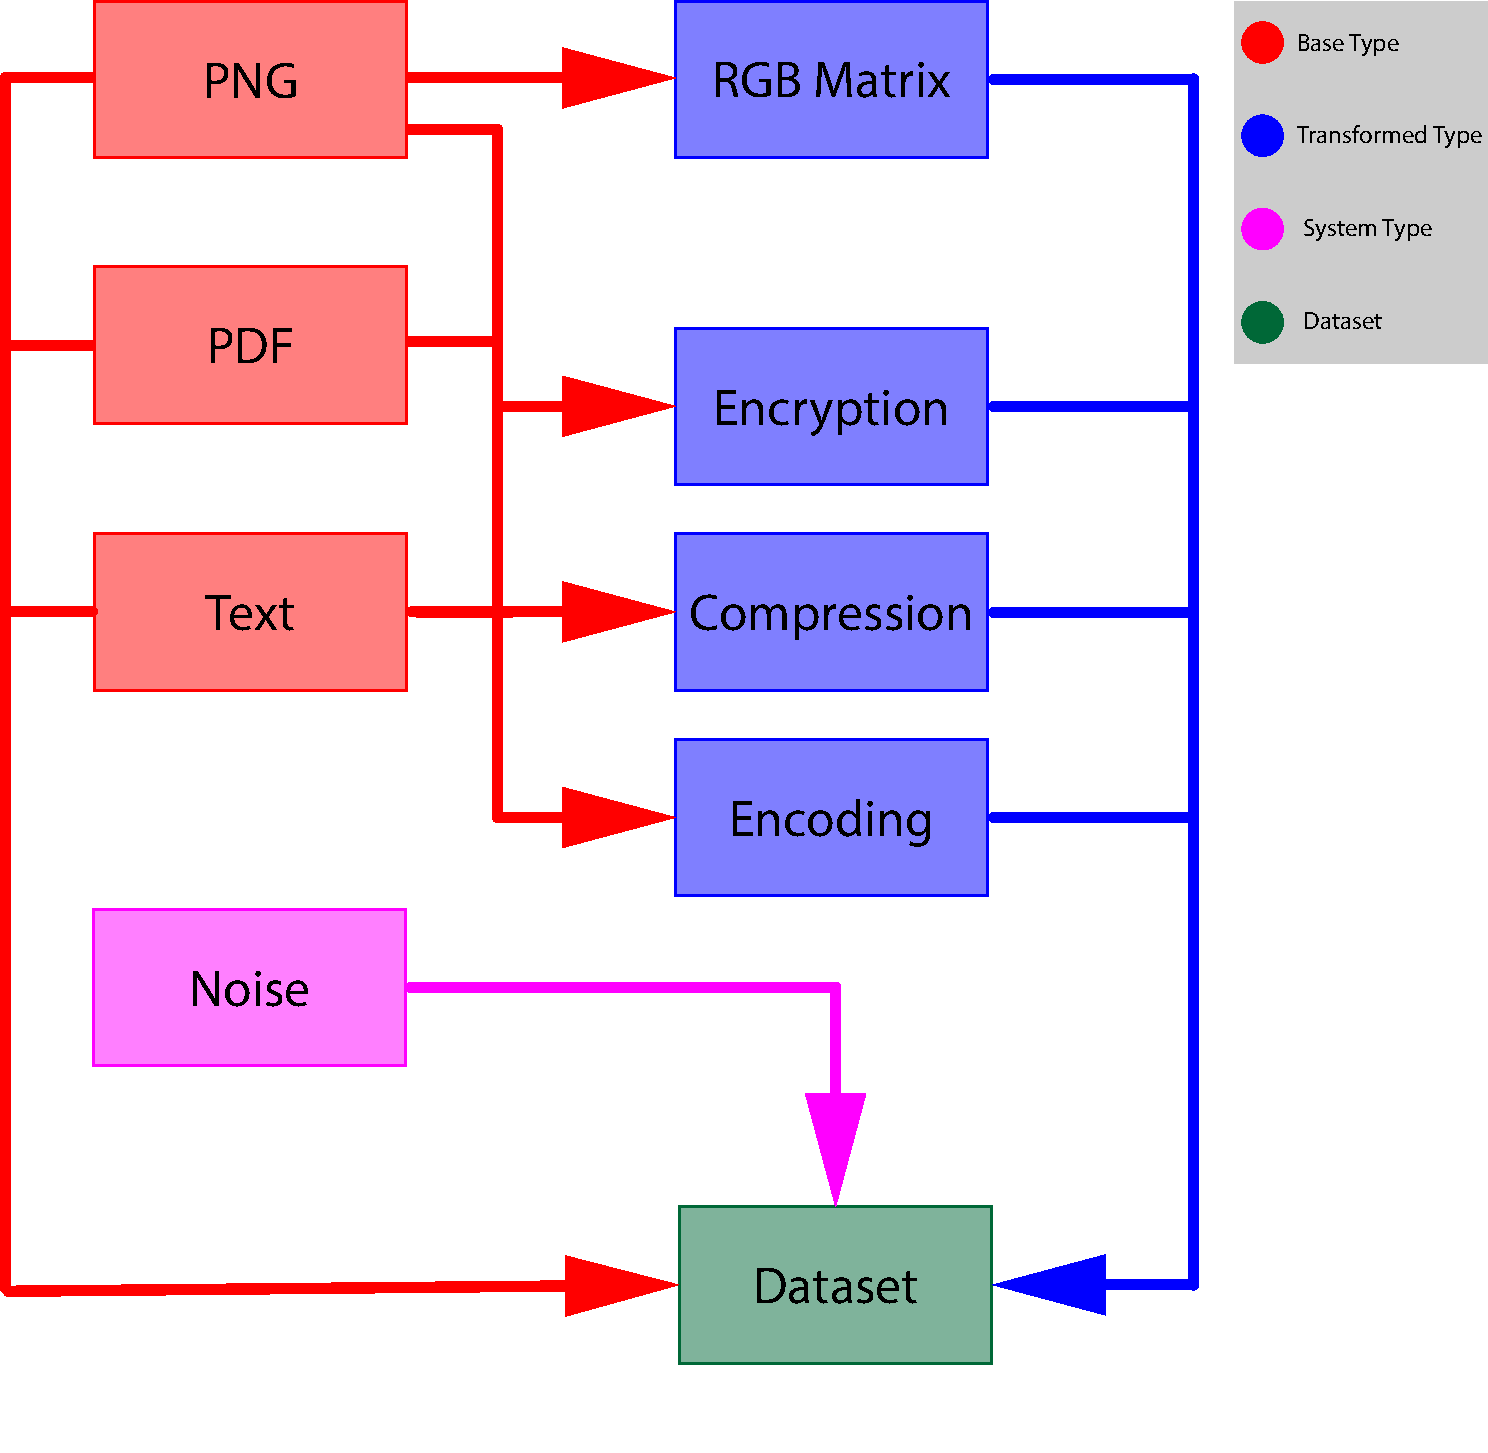
\includegraphics[width=0.5\textwidth]{tree.pdf} 
        \caption{Arbre représentatif des transformations}
    \end{figure}

    Nos jeux de données reposent sur une classification binaire distinguant les données chiffrées des données non chiffrées. Afin de simuler des dumps mémoire aussi réalistes et diversifiés que possible pour l'entraînement du modèle, ces deux classes principales englobent une multitude de sous-types. D'une part, la classe des données non chiffrées comprend du texte brut, des documents PDF, des images, des matrices de pixels, ainsi que des données ayant subi des transformations courantes (encodage Base64, algorithmes de compression à taux variables). À cela s'ajoutent du bruit aléatoire (noise) et des simulations d'en-têtes système. D'autre part, la classe chiffrée est exclusivement constituée de données traitées via l'algorithme AES, appliquées de manière aléatoire sur les formats sources précédemment cités (PDF, images, textes).

    \begin{figure}[H]
        \centering
        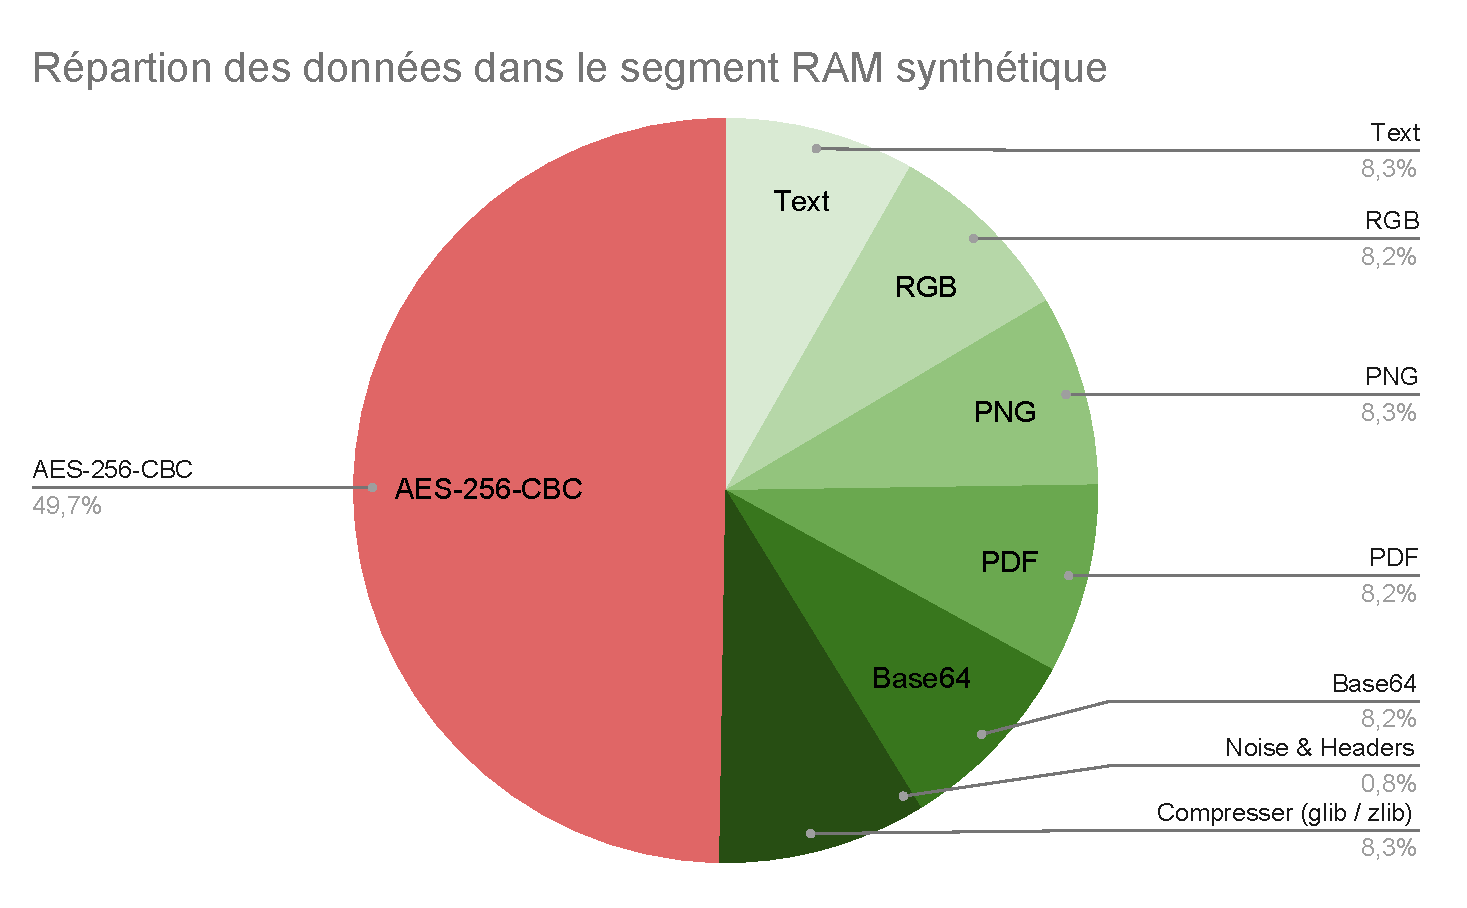
\includegraphics[width=0.7\textwidth]{repartRAM.pdf} 
        \caption{Répartition des données dans le dump mémoire synthétique}
    \end{figure}

    Afin de mener à bien l'apprentissage et l'évaluation du modèle, nous avons généré trois jeux de données distincts dédiés à l'entraînement, à la validation et au test. L'ensemble d'entraînement possède une taille de 1 Go, tandis que les ensembles de validation et de test mesurent 100 Mo chacun. Pour garantir une évaluation non biaisée, ces trois corpus partagent une distribution de classes strictement équilibrée, composée à 50 % de données chiffrées et à 50 % de données en non chiffrées.

    \section{Outils d'analyse}
    Pour faciliter l'interprétation des erreurs de classification et valider spatialement les prédictions du modèle, nous avons développé une interface de visualisation dédiée en React. Cet outil permet de confronter dynamiquement le dump binaire initial avec les fichiers de logs générés lors de l'inférence. En superposant les prédictions du Transformer à la "vérité terrain" (ground truth), nous pouvons identifier visuellement si les erreurs se concentrent sur des zones spécifiques, comme les transitions entre deux types de données ou les structures internes de certains fichiers.

    \section{Modèle de classification}
    \subsection{Introduction au modèle}

    \subsubsection{Transformers}
    L'architecture \textit{Transformer} représente un changement de paradigme majeur dans le domaine de l'apprentissage profond (Deep Learning). Introduit par \textit{Google} en 2017 à travers l'article \citefull{attention_is_all_you_need}, ce modèle s'est imposé comme le standard pour le traitement de données séquentielles, notamment dans le traitement automatique des langues (NLP).
    
    Contrairement aux architectures récurrentes conventionnelles (RNN et LSTM), qui opèrent par une analyse chronologique et itérative de l'information, le \textit{Transformer} repose sur un principe de parallélisation massive des flux de données.

    \subsubsection{Architecture Encodeur}
    Un encodeur traite et modélise l'information d'entrée en convertissant des données brutes en représentations vectorielles de haute dimension. Lorsqu'il est utilisé indépendamment d'un décodeur, ce module est particulièrement efficace pour les tâches de classification ou de compréhension sémantique, où la génération de texte n'est pas requise.
    \begin{figure}[H]
        \centering
        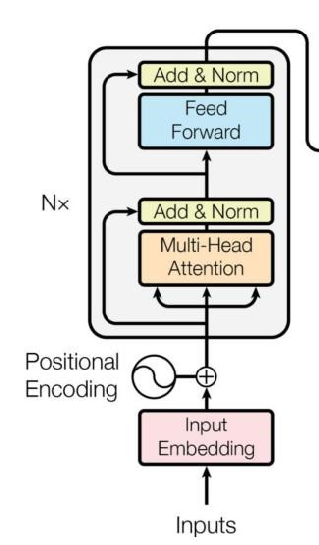
\includegraphics[width=0.3\textwidth]{architecture_encodeur.png} 
        \caption{Illustration d'un encodeur du papier \citefull{attention_is_all_you_need}}
    \end{figure}

    \subsubsection{Input Embedding}
    \textit{L'input embedding} transforme les données brutes en représentations vectorielles de dimension $d_{model}$, rendant l'information traitable mathématiquement par le modèle.

    Une fois projetés dans l'espace vectoriel, ces vecteurs sont multipliés par un facteur d'échelle $\sqrt{d_{model}}$ afin de stabiliser les gradients lors de l'entraînement.

    Contrairement aux réseaux récurrents (RNN), l'achitecture \textit{Transformer} traite les elements d'une séquence simultanément. Pour compenser cette absence de notion d'odre intrinsèque, un encodage de position est ajouté à chaque vecteur d'entrée. Cette information permet au modèle de distinguer la position relative de chaque element dans la séquence.

    Cet encodage repose sur des fonctions sinusoïdales de fréquences différentes, définies par les formules suivantes : 
    \begin{gather}
        PE_{(pos, 2i)} = \sin\left(\frac{pos}{10000^{2i/d_{model}}}\right) \\[10pt]
        PE_{(pos, 2i+1)} = \cos\left(\frac{pos}{10000^{2i/d_{model}}}\right)
    \end{gather}

    \subsubsection{Mécanisme d'attention}
    Le mécanisme de \textit{self-attention} permet au modèle de pondérer l'importance relative de chaque élément d'une séquence par rapport à tous les autres au sein de la même entrée. En projetant chaque token dans trois espaces distincts(Q, K, V), le modèle calcule une distribution de scores par produit scalaire. Cette opération permet d'extraire les dépendances contextuelles, qu'elles soient locales ou à longue distance, en focalisant le traitement sur les parties les plus informatives de la séquence.

    \begin{gather}
        \text{Attention}(Q, K, V) = \text{softmax}\left(\frac{QK^T}{\sqrt{d_k}}\right)V \\[10pt]
        Q = \text{matrice de requêtes} \nonumber \\
        K = \text{matrice de clés} \nonumber \\
        V = \text{matrice de valeurs} \nonumber \\
        d_k = \text{dimension des clés} \nonumber
    \end{gather}

    L'attention multi-têtes, c'est l'application de plusieurs mécanismes de \textit{self-attention} en parallèle, dans le but de spécifier et d'extraire plusieurs métriques (types, syntaxe …) afin de ne pas écarter de sens exploitable. Leurs résultats sont donc fusionnés pour extraire un unique vecteur portant toutes les informations sur le sens.

    \subsubsection{Sortie du modèle}
    A la sortie du modèle on trouve des logits (score une valeur entre $-\infty$ et $+\infty$), nous y appliquons une fonction sigmoïde pour \textit{Transformer} entre 0 et 1, entre les deux classes.
    \begin{equation}
        \sigma(x) = \frac{1}{1 + e^{-x}}
    \end{equation}

    \section{\texttt{BytesTransformerClassifier}}
    \begin{figure}[H]
        \centering
        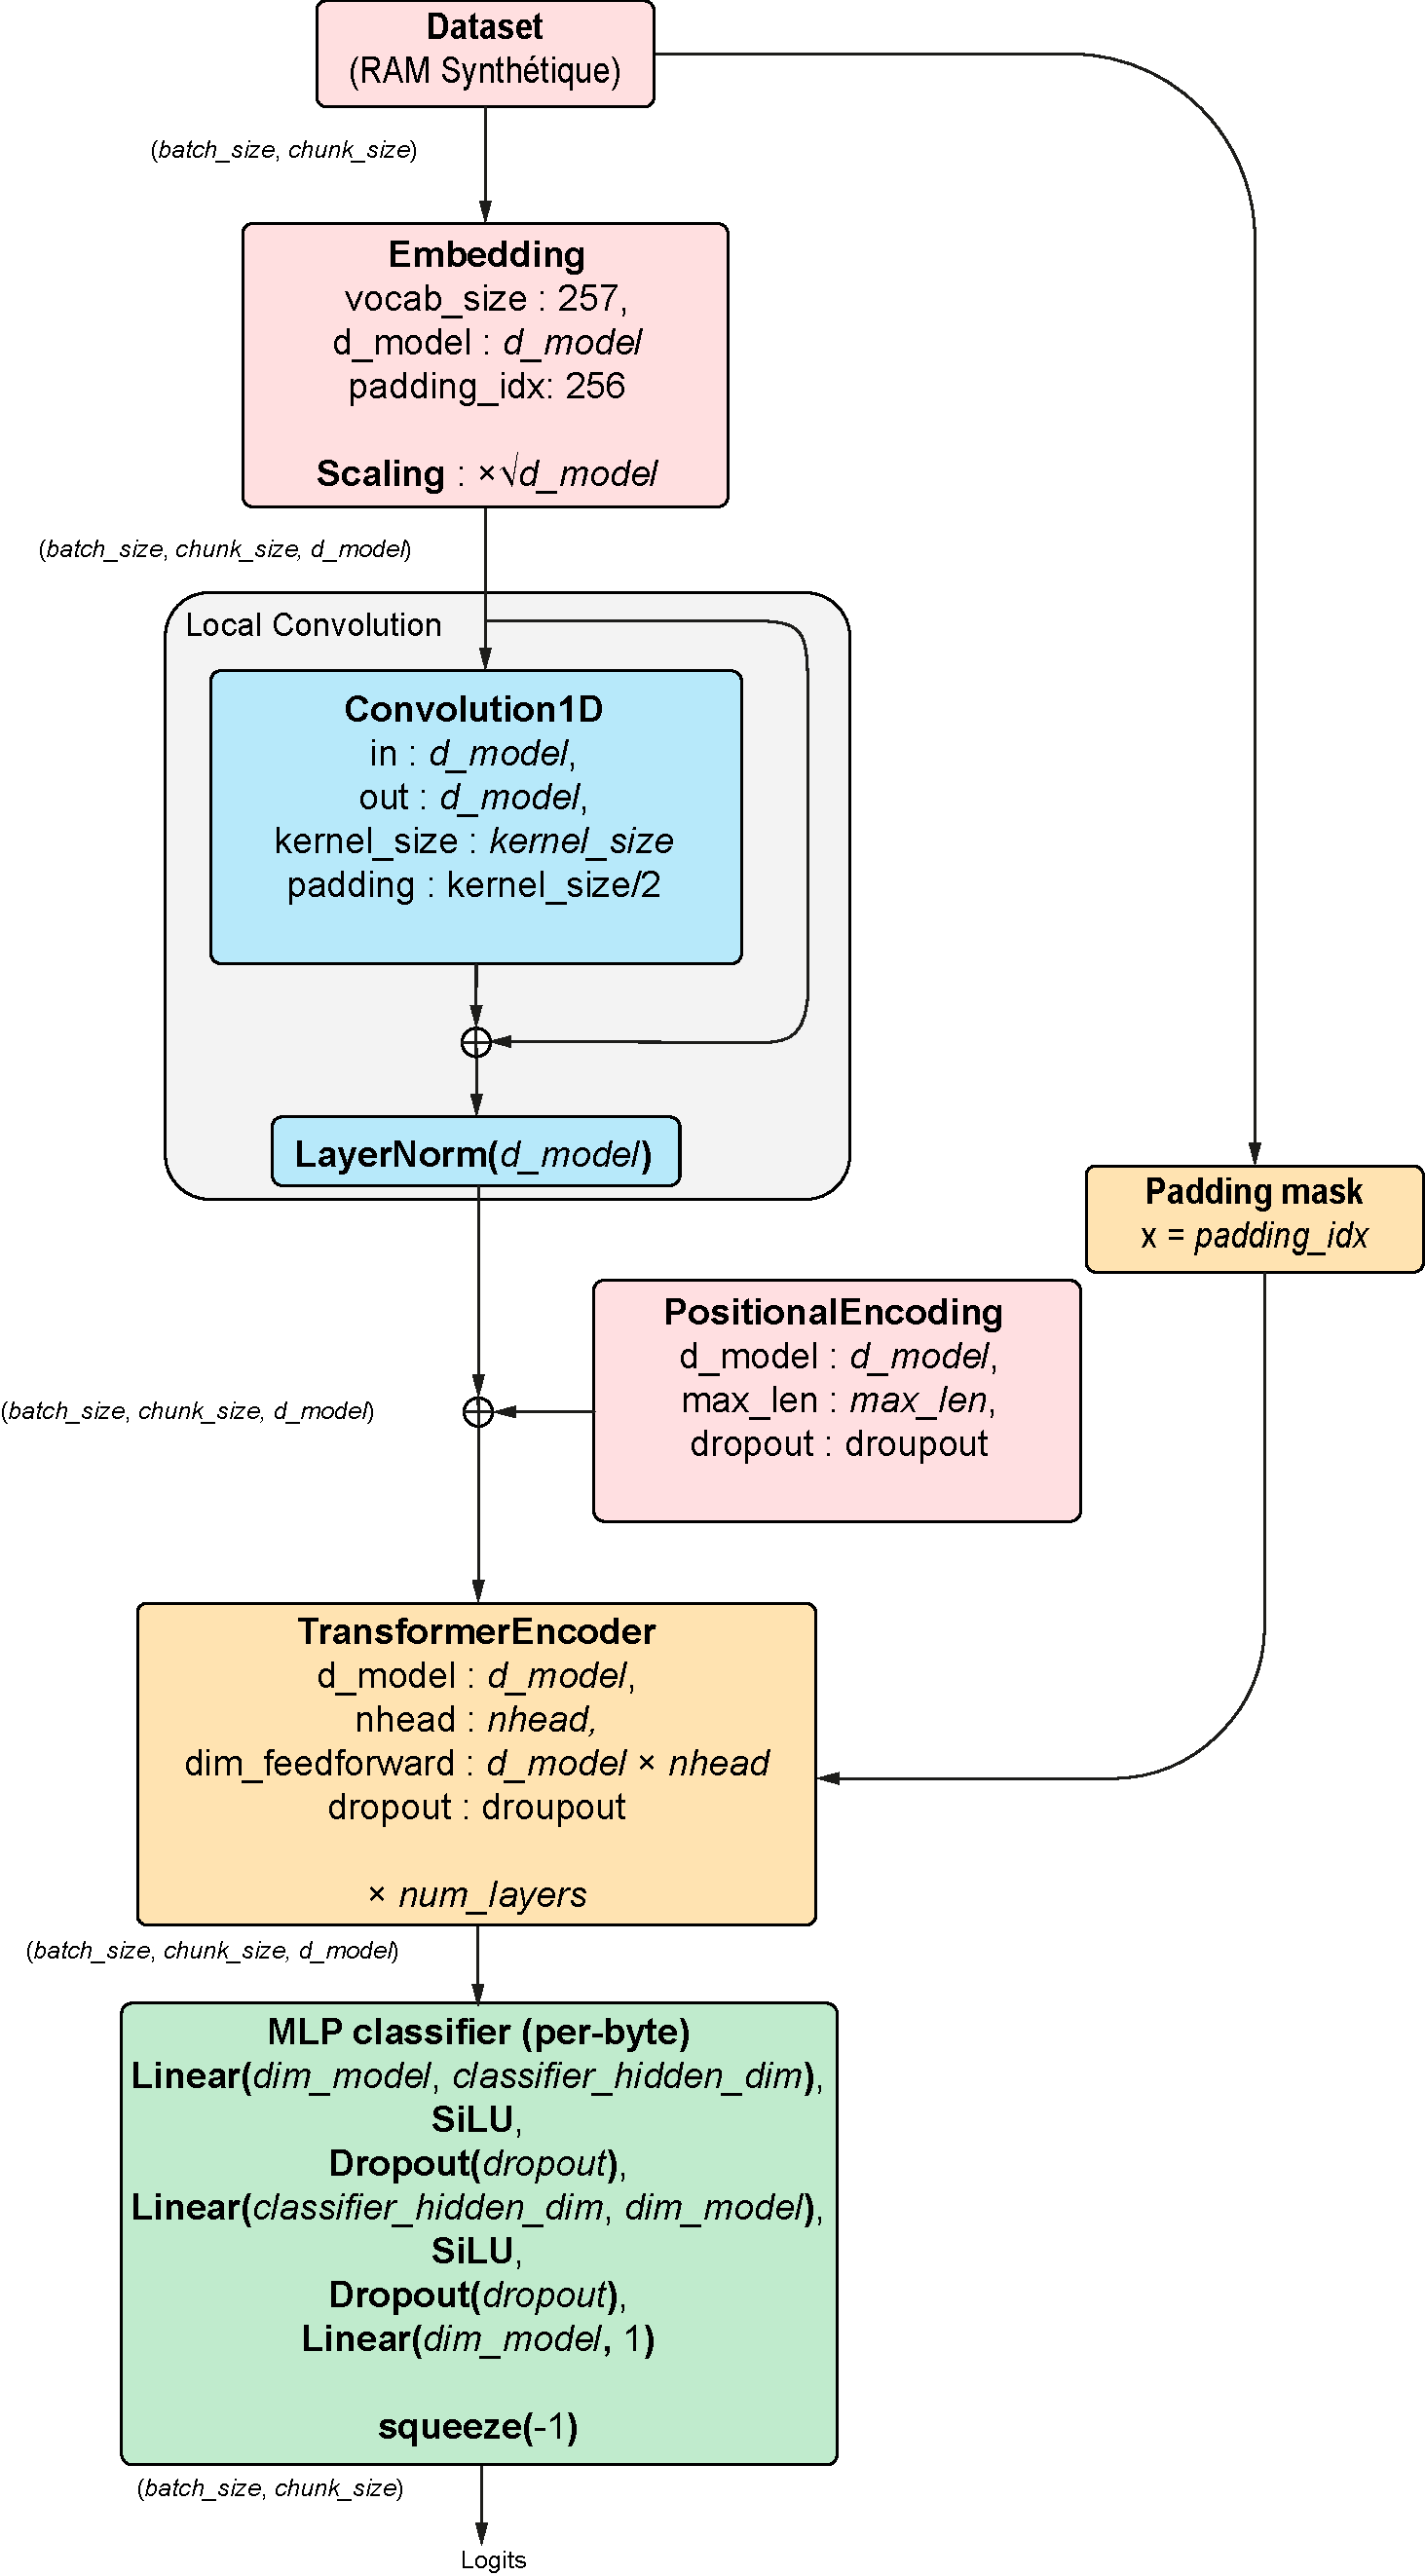
\includegraphics[width=0.7\textwidth]{transformerPipeline.pdf} 
        \caption{Pipeline de classification du \texttt{BytesTransformerClassifier}}
    \end{figure}


    \section{Entraînement et validation}
    \begin{figure}[H]
        \centering
        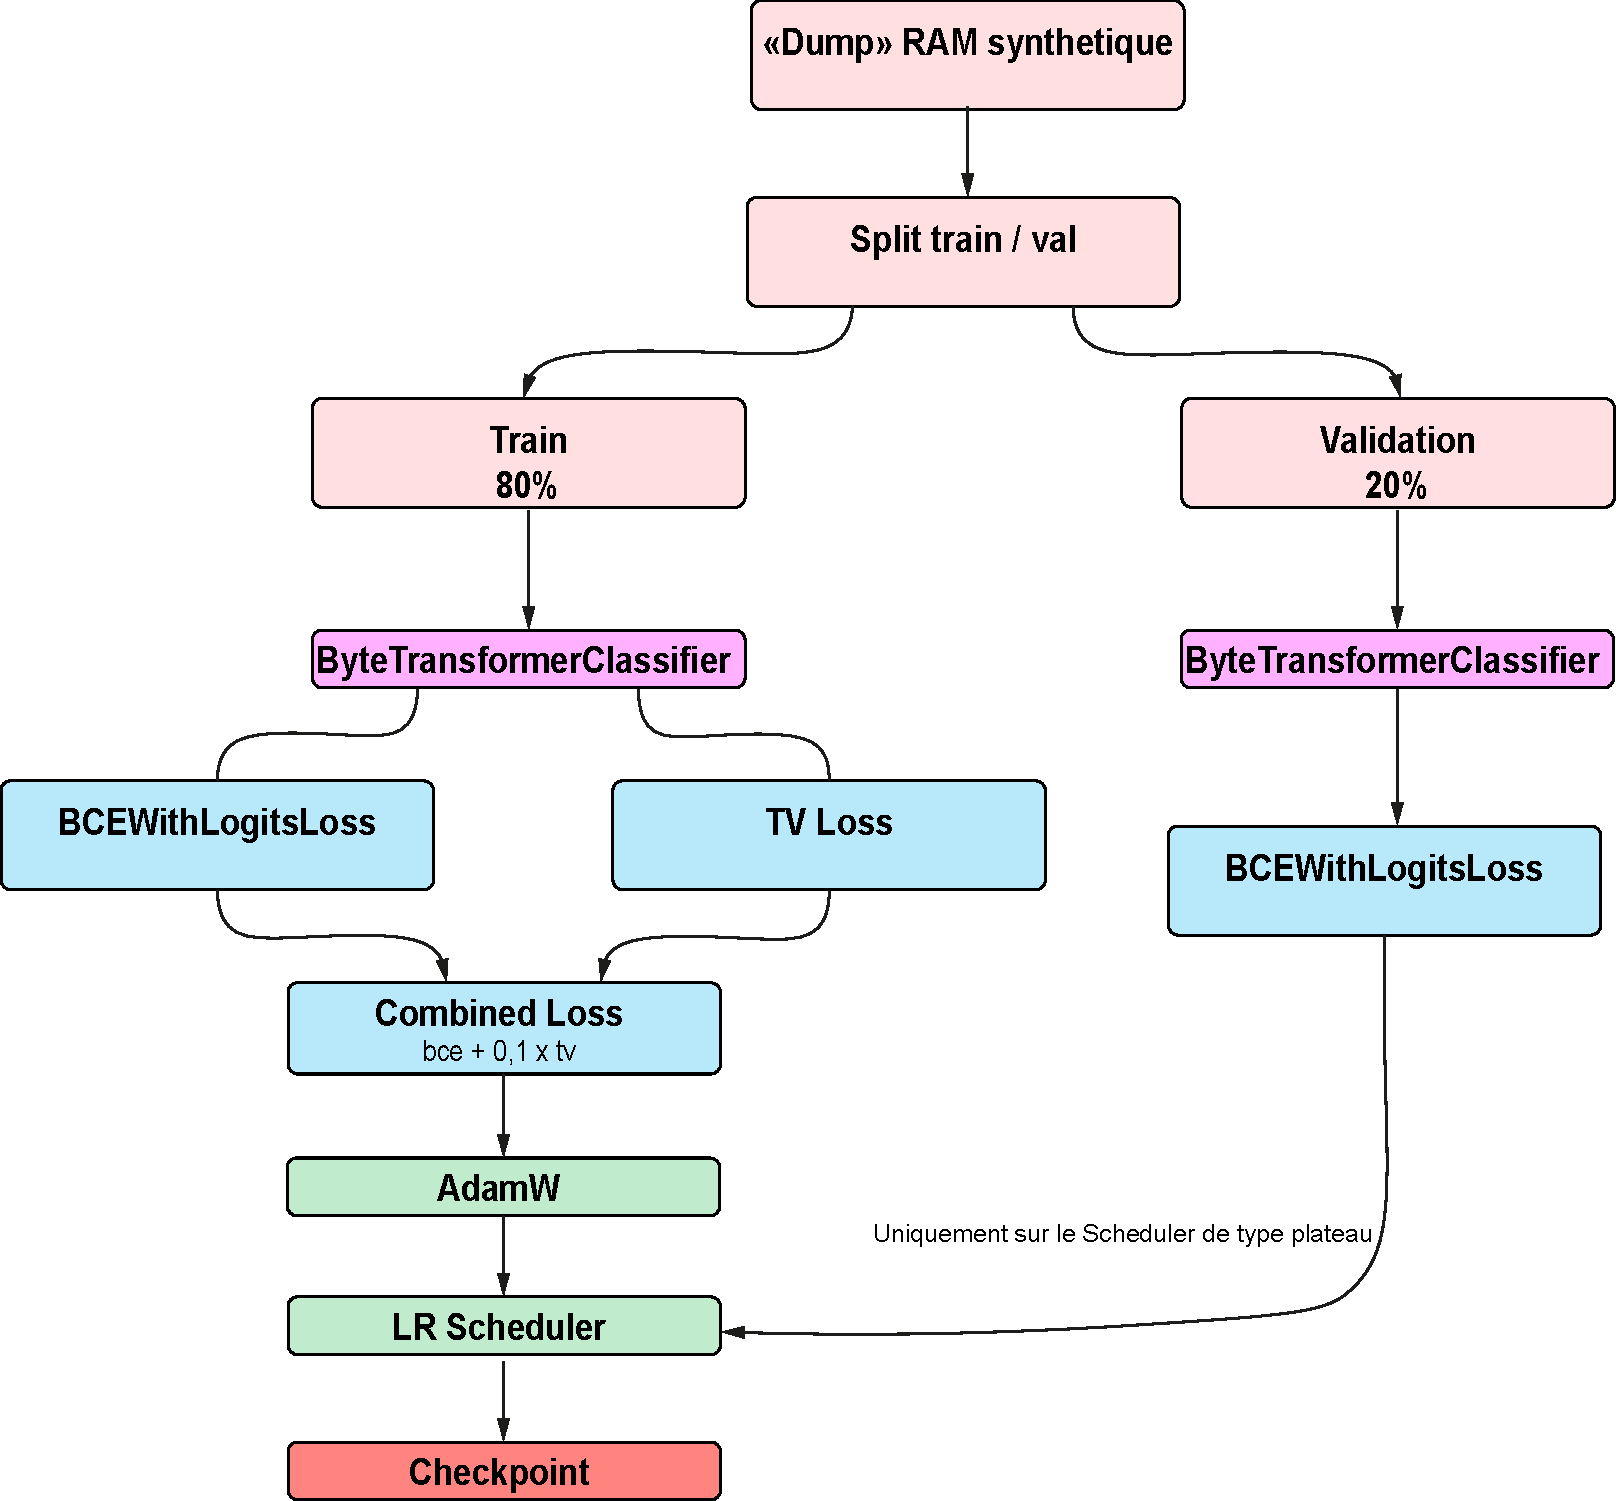
\includegraphics[width=1\textwidth]{trainningPipeline.pdf} 
        \caption{Illustration d'un encodeur du papier \citefull{attention_is_all_you_need}}
    \end{figure}

    Nous utilisons \texttt{BinaryCrossEntropy}. Ce choix est justfié car nous classifions chaque octet entre deux classes (chiffré ou non chiffré).
    
    Les paramètres du modèle sont optimisés via AdamW, configuré avec un \textit{weight decay} de $1e-2$ ainsi que le \textit{learning rate} de $1e-4$ afin de régulariser l'apprentissage sur les 1 Go de données synthétiques. Cet optimiseur permet de naviguer efficacement dans l'espace de haute dimension généré par le mécanisme de self-attention.

    \section{Principe de \textit{l'overlapping} (recouvrement)}
    Le modèle traite le dump mémoire par fenêtres glissantes de \texttt{N} octets. Au lieu de découper la mémoire en blocs contigus, nous utilisons un pas de glissement (stride) inférieur à la taille de la fenêtre. Par conséquent, chaque octet de la RAM est analysé plusieurs fois par le Transformer, au sein de contextes différents.
    \begin{figure}[H]
        \centering
        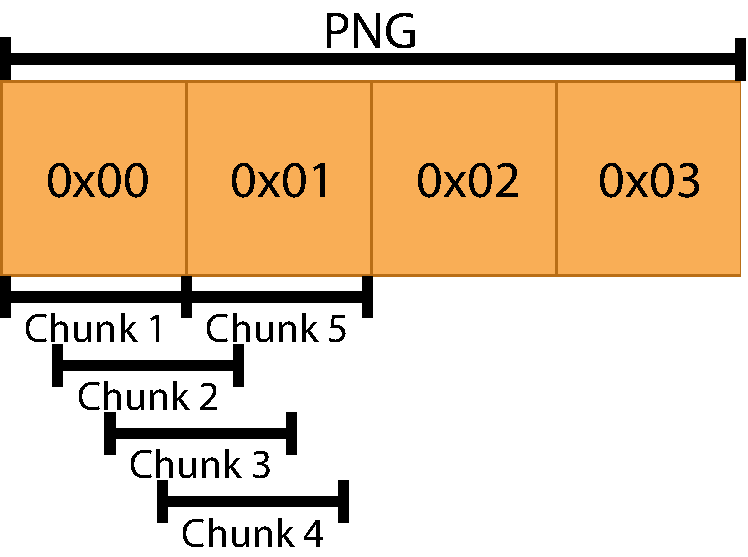
\includegraphics[width=0.5\textwidth]{chunk.pdf} 
        \caption{Illustration du principe de l'overlapping, ici avec un stride de $\frac{1}{4}$ de chunk}
    \end{figure}

    \section{Pipeline de vote pondéré}
    Après avoir transformé les logits en probabilités via une fonction sigmoïde, les prédictions locales sont agrégées. Cette étape repose sur une pondération de chaque résultat par le score de confiance associé.
    \begin{gather}
        \text{Confiance}_x = 2 \times |p_x - 0.5| \\[10pt]
        \text{P\_Global}_x = \frac{\sum_{i=1}^{n} \text{Confiance}_i \times p_i}{\sum_{i=1}^{n} \text{Confiance}_i} \\[6pt]
        \text{\small avec } n = \frac{\text{chunk\_size}}{\text{stride}} \nonumber
    \end{gather}

    \chapter{Résultats}
    \section{Performance Globales}
    \begin{table}[H]
        \centering
        \begin{tabular}{|c|c|}
            \hline
            Métrique finale & Score \\
            \hhline{|=|=|}
            Accuracy & $1$ \\
            \hline
            Precision & $1$ \\
            \hline
            Recall & $1$ \\
            \hline
            F1-Score & $1$ \\
            \hline
        \end{tabular}
        \caption{Performances globales du classifieur RAID}
    \end{table}

    Matrice de confusion :

    \section{Courbes d'apprentissage}
        \begin{figure}[H]
            \centering
            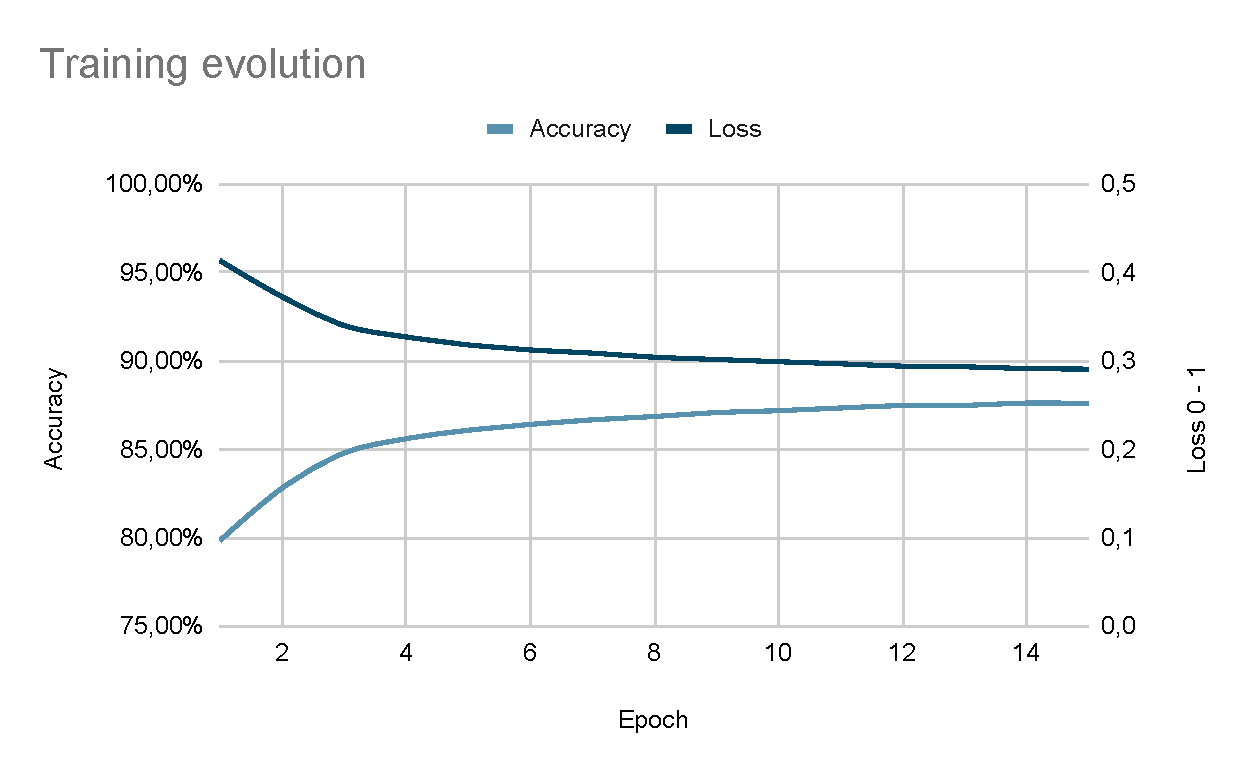
\includegraphics[width=0.7\textwidth]{learningCurves.pdf} 
            \caption{Courbes d'apprentissage du modèle}
        \end{figure}


    \chapter{Discussion}
    \section{Performance du vote pondéré}
    L'un des défis majeurs de l'analyse de dumps mémoire par un \textit{Transformer} réside dans la volatilité des prédictions locales. Un segment de données peut présenter des caractéristiques ambiguës (par exemple, un en-tête de fichier compressé ressemblant à du texte structuré) qui induisent le modèle en erreur s'il est analysé de manière isolée. 

    Pour pallier cette limite, nous avons implémenté un mécanisme de vote pondéré. Cette approche permet de stabiliser les prédictions et d'augmenter la fiabilité de la classification des zones de mémoire.

	En confrontant plusieurs prédictions pour un même octet via des fenêtres glissantes, nous avons observé une réduction des “artefacts de prédiction" (changements de classe abrupts et incohérents sur quelques octets). Cette approche agit comme un filtre passe-bas, éliminant le bruit haute fréquence dans les résultats pour ne conserver que les zones où le modèle maintient une confiance élevée et constante.  

    Il est important de noter que cette robustesse a un coût. L'utilisation d'un \textit{stride} (pas) réduit pour multiplier les votes multiplie proportionnellement le temps d'inférence. Dans des grands volumes de données, ce compromis entre le temps d'analyse et la précision de la segmentation est un paramètre critique. Nos résultats suggèrent que le gain en fiabilité justifie cette latence, tout en ouvrant la porte à des optimisations futures sur le parallélisme de l'agrégation des votes.

    \section{Chiffrement et compression : l'entropie trompe le modèle}
    L'analyse des erreurs de classification révèle une confusion récente du modèle entre les segments de données chiffrés et compressés. Cette difficulté s'explique par la nature mathématique même des algorithmes utilisés dans le projet, tels que l'AES-256-CBC pour le chiffrement et zLib ou Gzip pour la compression.

    \subsection{La convergence statistique des hautes entropies}
    Le modèle \textit{Transformer} repose sur sa capacité à identifier des structures et des dépendances au sein des séquences d'octets. Or, l'objectif d'un algorithme de compression efficace est d'éliminer toute redondance, ce qui conduit à une distribution des octets proche d'un bruit blanc aléatoire, simulant ainsi une entropie maximale. Le chiffrement et la compression sont deux processus produisent des flux binaires dépourvus de motifs répétitifs exploitables par les mécanismes d'attention du modèle.

    \subsection{Impact sur la précision de la segmentation}
    Dans les résultats d'évaluation, cette confusion se traduit par des faux positifs où des flux compressés sont étiquetés comme \texttt{ENCRYPTED}. Les résultats montrent que même avec une validation par vote pondéré, le score de confiance reste souvent élevé pour ces deux catégories, car le modèle "est certain" de ne pas faire face à du texte ou des images structurées, mais ne possède pas de descripteurs sémantiques suffisants pour distinguer un flux compressé d'un flux chiffré.

    \subsection{Limites de l'approche sémantique pure}
    Cette problématique souligne une limite intrinsèque de l'apprentissage profond appliqué aux flux binaires bruts : sans la détection de signatures spécifiques (headers)  que le projet cherche justement à éviter pour gagner en généricité, la distinction entre haute entropie "utile" (compression) et "intentionnelle" (chiffrement) demeure un défi ouvert. Pour les travaux futurs, l'intégration de métriques statistiques complémentaires, telles que des tests de distribution de fréquences bien plus fins au sein des couches du classifieur, pourrait offrir une piste pour séparer ces deux types de données

    \section{Signatures Statiques {\small vs} Apprentissage Profond}
    L'approche conventionnelle sur ce type de tâches repose largement sur l'utilisation de signatures statiques (comme les magic bytes) ou l'analyse de structures de fichiers connues. Cependant, le projet R.A.I.D. démontre qu'une approche basée sur l'apprentissage profond, et plus spécifiquement sur les architectures \textit{Transformers}, offre une flexibilité que les outils traditionnels pourraient peiner à atteindre.

    \subsection{Sémantique binaire {\small vs} Identification rigide}
    Les méthodes classiques échouent lorsque les données sont fragmentées ou dépourvues de leurs en-têtes originaux, une situation fréquente au sein d'un dump RAM. Là où un outil statique verrait une suite d'octets incohérente, le modèle parvient à extraire une "signature statistique" du contenu. En apprenant la sémantique profonde des différents types de données (la structure d'un texte, la distribution d'une image compressée), le \textit{Transformer} identifie la nature de l'information même en l'absence de métadonnées explicites.

    \subsection{Résilience face à l'obfuscation}
    Une limite majeure des signatures statiques réside dans leur vulnérabilité aux techniques d'obfuscation simples. Un changement mineur dans les premiers octets d'un fichier suffit à tromper un scanner traditionnel. À l'inverse, l'utilisation du mécanisme d'attention du \textit{Transformer} permet au modèle de pondérer l'importance de chaque octet dans son contexte global. Cette capacité rend le système beaucoup plus résilient : la classification ne repose pas sur un point de passage unique, mais sur une compréhension diffuse du bloc de données de 512 octets.

    \subsection{Le coût de l'intelligence}
    Il est toutefois nécessaire de nuancer cette supériorité par le coût computationnel associé. Si les signatures statiques sont quasi instantanées et légères, l'inférence d'un modèle Transformer couplée à une stratégie de vote pondéré, exige des ressources matérielles significatives (GPU). Cette discussion souligne un arbitrage nécessaire : les méthodes classiques restent d'une utilité majeure en l'absence de matériel performant ou lors d'analyses ou l'on cherche la rapidité brute.

    \section{Limites}
    \subsection{La généralisation face aux données réelles}
    Bien que les résultats soient prometteurs, il est important de souligner que le modèle a été entraîné et évalué sur un jeu de données synthétique. Bien que ce dernier s'efforce de reproduire la diversité d'un dump mémoire, il existe inévitablement des écarts avec la complexité d'une mémoire vive réelle, notamment au niveau de la fragmentation dynamique et des structures de données propriétaire liées aux OS.

    On peut aussi considérer que dans la RAM, la présence de formats propriétaires non inclus dans le dataset pourraient faire l'objet d'erreurs de classification si leur format paraît trop éloigné de la signature statistique des données présentes dans le corpus d'entraînement. La non exhaustivité des types présents dans notre dataset peut donc influencer négativement les performances de la classification du modèle.

    \chapter{Conclusion}
    Le projet R.A.I.D. (RAM Artificial Inspection Dump) s'affranchit des méthodes traditionnelles basées sur des signatures statiques, cela démontre la viabilité des architectures de type \textit{Transformer} pour l'interprétation sémantique de flux binaires bruts.
    \\

    À travers le développement d'un pipeline complet, de la génération synthétique de dumps complexes à l'implémentation du \texttt{BytesTransformerClassifier}, nous avons validé l'hypothèse selon laquelle l'entropie et la prédictibilité des données sont des descripteurs puissants pour la segmentation mémoire. Le modèle a prouvé sa capacité à distinguer avec précision les zones chiffrées des structures de données textuelles ou visuelles, et ce, sans connaissance préalable des formats de fichiers.

    La réussite de ce travail réside aussi dans la stratégie de vote pondéré, qui permet de transformer des prédictions locales incertaines en une segmentation globale robuste. Toutefois, des défis subsistent, notamment la distinction entre la forte compression (haute entropie) et le chiffrement, ainsi que l'optimisation des ressources pour traiter des dumps de grande échelle en temps réel.
    \\
    
    Les résultats obtenus ouvrent des voies pour la recherche au sein de l'équipe SAFE du GREYC. L'intégration de ce modèle dans un outil d'expertise visuelle, couplée à un passage vers un apprentissage non supervisé sur des dumps système réels, permettra de poser des bases vers une assistance automatisée complète pour les enquêteurs numériques. À terme, R.A.I.D. pourrait devenir une brique logicielle pour les travaux de reconstruction automatique d'artefacts volatils, ou l'extraction de données exploitables depuis de véritables dumps de RAM.


    \printbibliography[title={Bibliographie}, heading=bibintoc]

\end{document}